\subsection{Debayering}
Debayering is the process of estimating complete color information for an image that has been captured through a \gls{cfa}, particularly on the Bayer pattern \cite{getreuerMalvarHeCutlerLinearImage2011}.
In the Bayer pattern, green pixels cover half the array in a lattice, and the red and blue pixel locations are spaced uniformly every two pixels shown in figure \ref{fig:debayer:bayer_pattern} \cite{getreuerMalvarHeCutlerLinearImage2011}.
Different orderings of the colors exists, with the most common ones being RGGB, BGGR, GRBG, and GBRG, but the concepts stays the same.

Debayering involves interpolating the missing color information from the \gls{cfa} data.
Malvar, He, and Cutler proposed a simple linear method using 5 x 5 filters that shows surprisingly good results \cite{getreuerMalvarHeCutlerLinearImage2011}.
The method they present is derived as a modification of bilinear interpolation, and it involves adding Laplacian cross-channel corrections to improve the quality of the bilinear method.
The demosaicking is implemented by convolution with a set of linear filters, and there are eight different filters for interpolating the different color components at different locations as can be shown in figure \ref{fig:debayer:malvar_filters}.
The method is more suited for parallel execution than many others as discussed in \todo.


\begin{figure}[tb]
    \centering
    \begin{tabular}[b]{ccc}
        \subcaptionbox{RGGB bayer pattern}{
            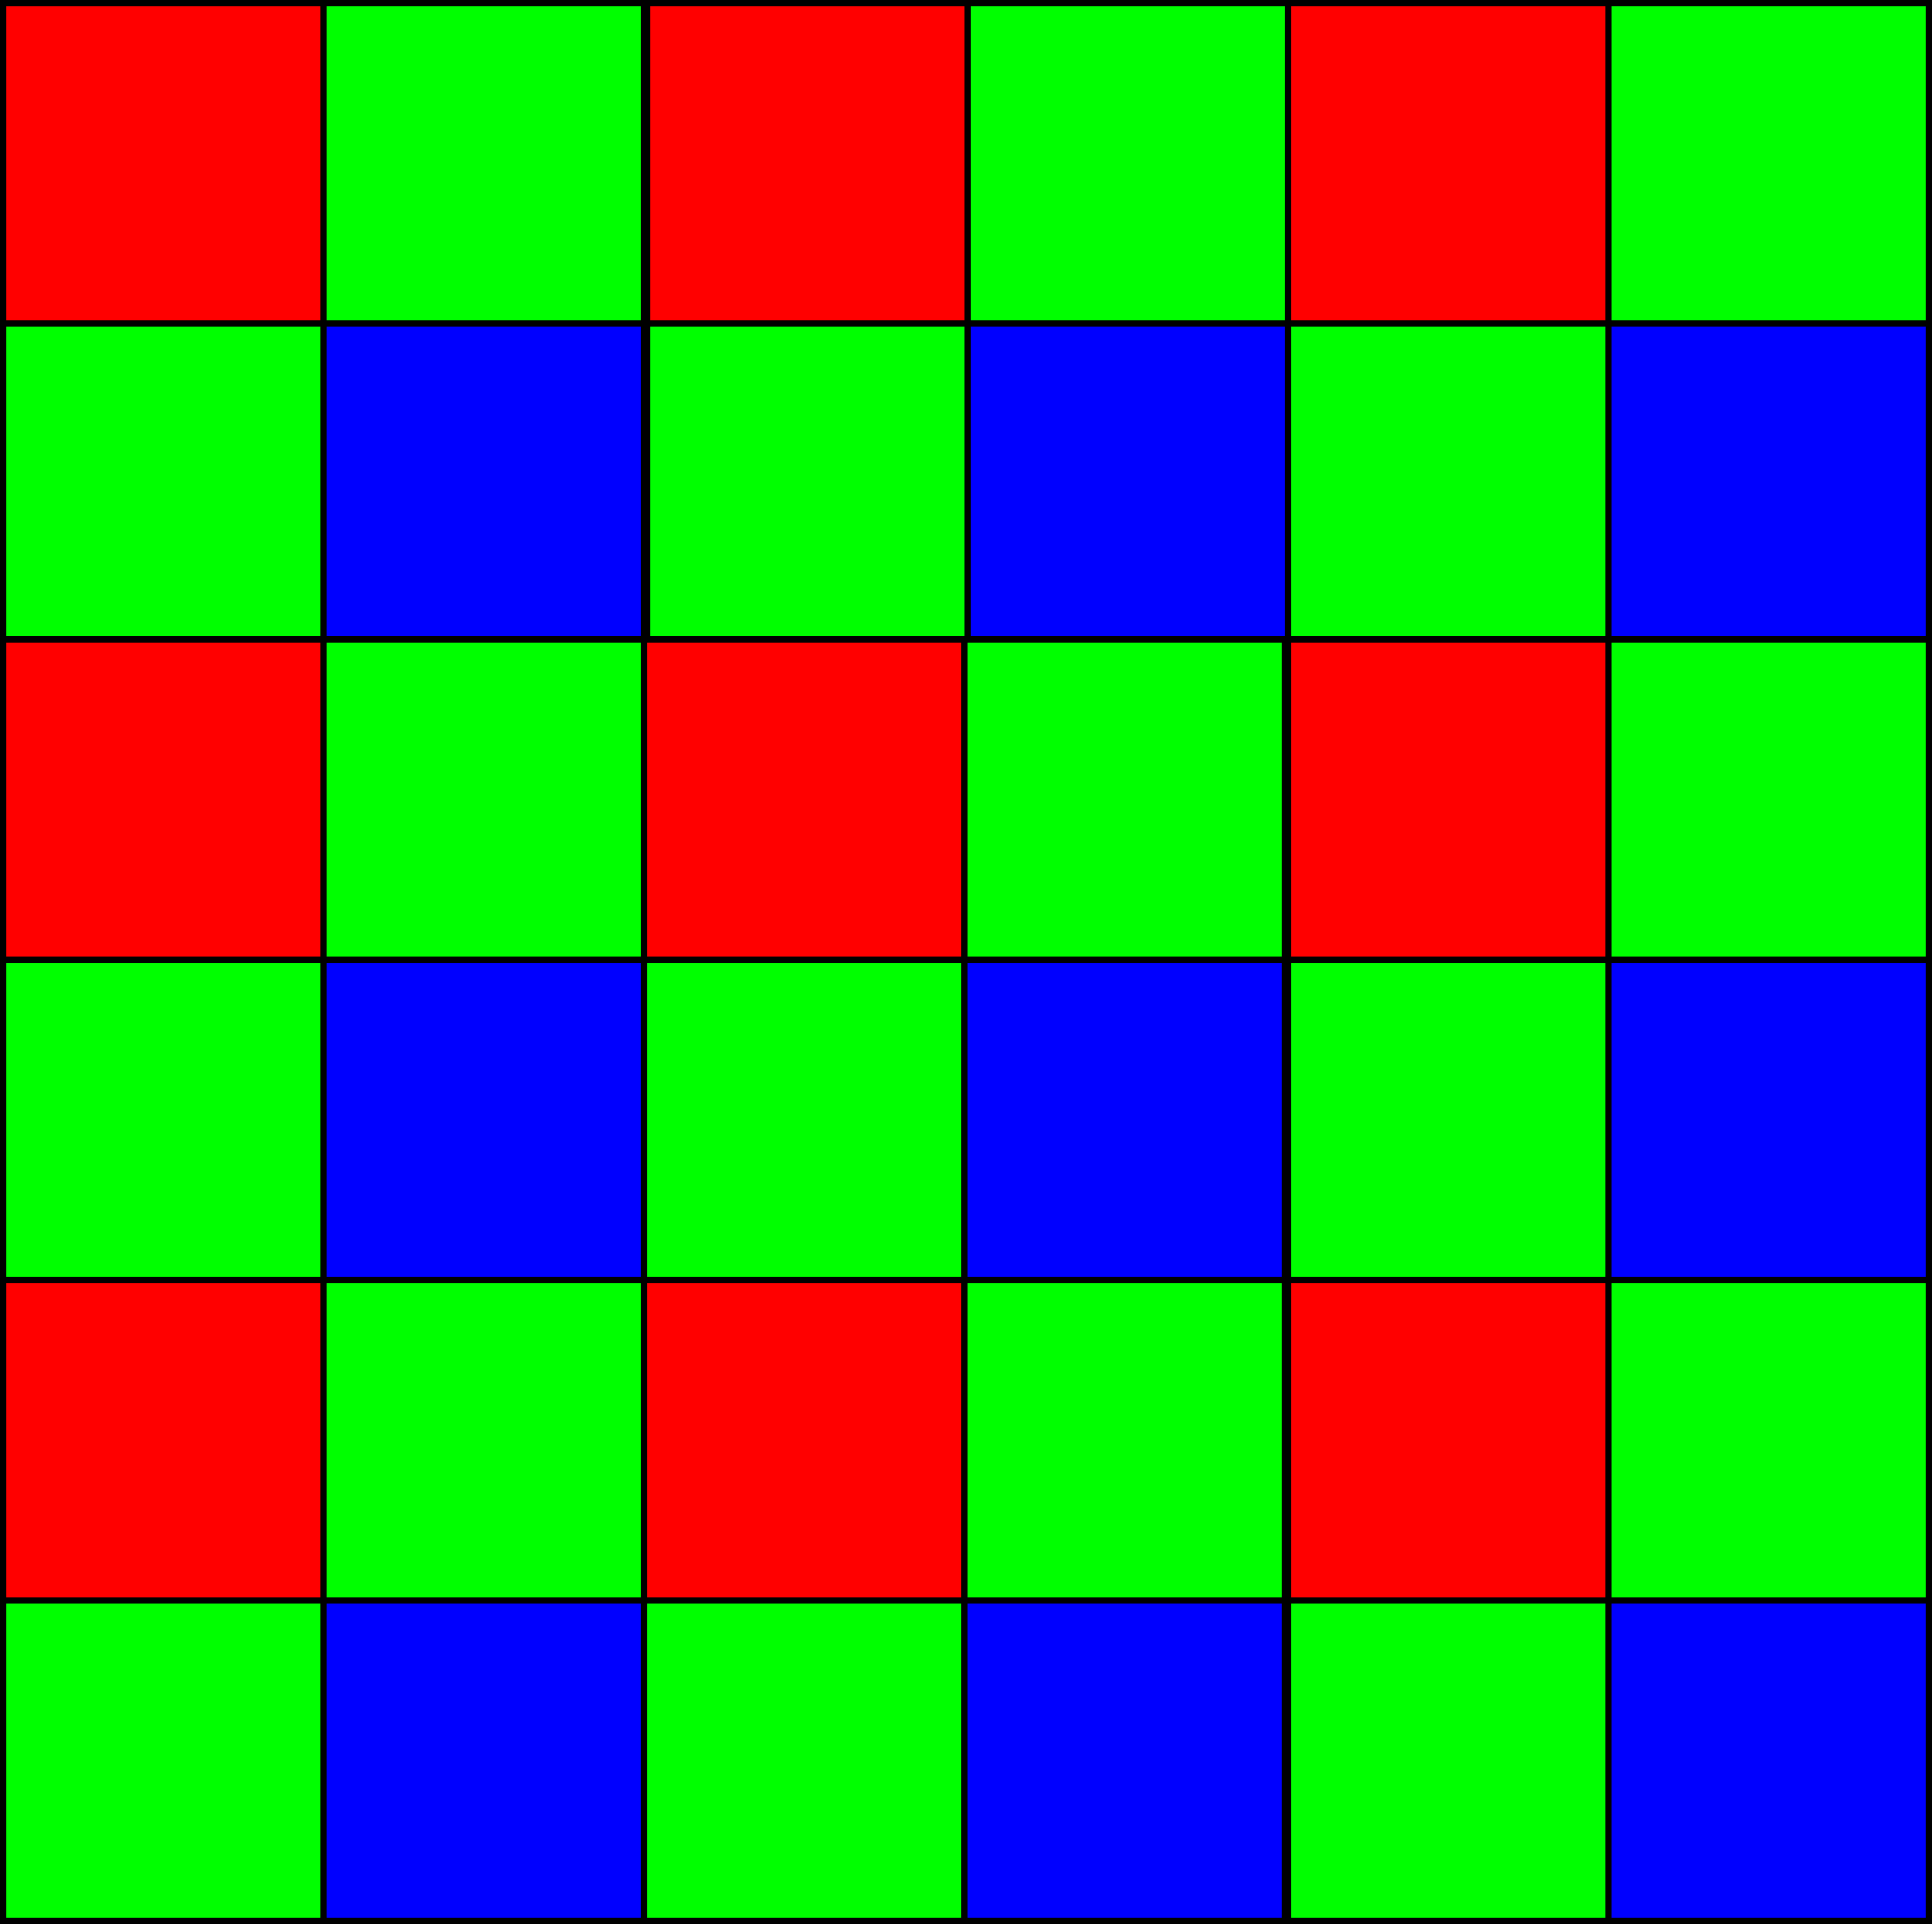
\includegraphics[width=0.25\textwidth]{figures/debayer/bayer_pattern.pdf}
            \label{fig:debayer:bayer_pattern}
        } &
        \subcaptionbox{Green at red}{
            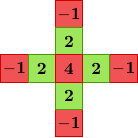
\includegraphics[width=0.25\textwidth]{figures/debayer/g_at_r.png}
        } &
        \subcaptionbox{Green at red}{
            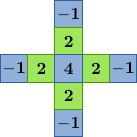
\includegraphics[width=0.25\textwidth]{figures/debayer/g_at_b.png}
        }
        \\
        \subcaptionbox{Red at }{
            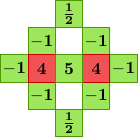
\includegraphics[width=0.25\textwidth]{figures/debayer/r_at_g_rr.png}
        } &
        \subcaptionbox{Red at green, blue row}{
            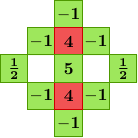
\includegraphics[width=0.25\textwidth]{figures/debayer/r_at_g_br.png}
        } &
        \subcaptionbox{Red at blue}{
            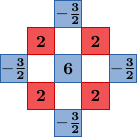
\includegraphics[width=0.25\textwidth]{figures/debayer/r_at_b.png}
        }
        \\
        \subcaptionbox{Blue at green, red row}{
            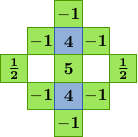
\includegraphics[width=0.25\textwidth]{figures/debayer/b_at_g_rr.png}
        } &
        \subcaptionbox{Blue at green, blue row}{
            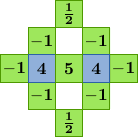
\includegraphics[width=0.25\textwidth]{figures/debayer/b_at_g_br.png}
        } &
        \subcaptionbox{Blue at red}{
            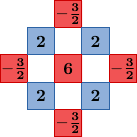
\includegraphics[width=0.25\textwidth]{figures/debayer/b_at_r.png}
        }
    \end{tabular}
    \caption{Coefficient values used by Malvar-He-Cutler scaled by 8 \cite{getreuerMalvarHeCutlerLinearImage2011}\cite{CommonsBayerPattern2020}}
    \label{fig:debayer:malvar_filters}
\end{figure}

\begin{figure}[tb]
    \centering
    \begin{tabular}[b]{ccc}
        \subcaptionbox{Exact image}{
            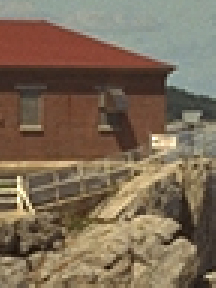
\includegraphics[width=0.3\textwidth]{figures/debayer/house_orig.jpg}

        } &
        \subcaptionbox{Observed Image}{
            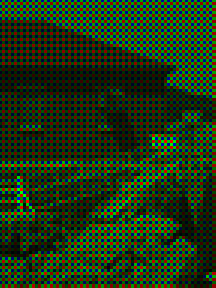
\includegraphics[width=0.3\textwidth]{figures/debayer/house_bayer.png}
        }
        \\
        \subcaptionbox{Bilinear (PSNR=25.61)}{
            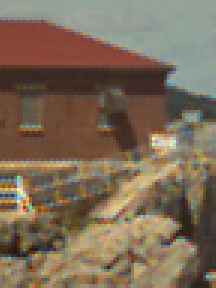
\includegraphics[width=0.3\textwidth]{figures/debayer/house_bilinear.png}
        } &

        \subcaptionbox{Hamilton-Adams \todo (PSNR=31.62)}{
            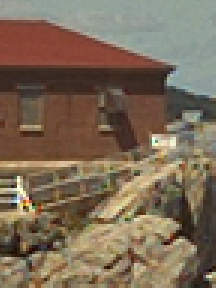
\includegraphics[width=0.3\textwidth]{figures/debayer/house_hamilton.png}
        } &
        \subcaptionbox{Malvar-He-Cutler (PSNR=31.15)}{
            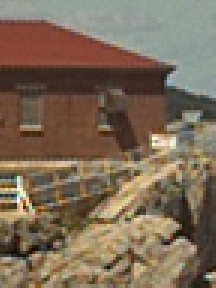
\includegraphics[width=0.3\textwidth]{figures/debayer/house_malvar.png}
        }
    \end{tabular}
    \caption{Coefficient values used by Malvar-He-Cutler scaled by 8 \cite{getreuerMalvarHeCutlerLinearImage2011}}
\end{figure}
\chapter{Debayer}
This chapter will discuss how a custom debayer algorithm was developed in \cuda.


% \subsection{__half2}
\subsection{Unpacking}
The \lucid cameras are capable of
\begin{figure}
    \centering
    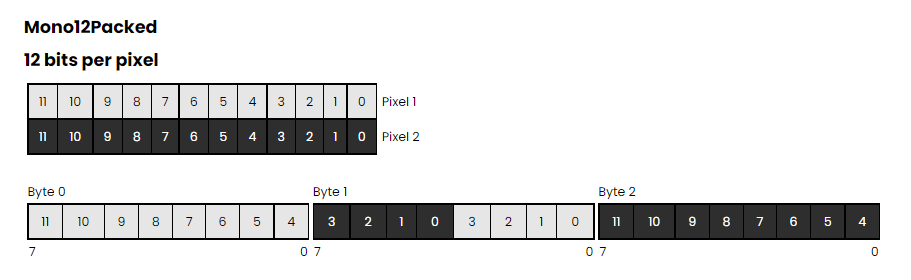
\includegraphics[width=\textwidth]{figures/Mono12Packed.png}
    \caption{Bit layout of the \cite{fisherRe15406LUT2023}}
    \label{fig:mono12packed}
\end{figure}

\begin{listing}[H]
    \begin{minted}{cuda}
        template <int width, int width_in>
        __device__ __forceinline__ void unpack10(__half2 *work_row, 
                                                 const unsigned int *img_row,
                                                 int tx) {
            __half2 *const out = &work_row[tx * 8 + 2];
        
            if (tx * 5 < width_in) {
                unsigned int buf_a, buf_b;
                buf_a = img_row[tx * 5];
                buf_b = img_row[tx * 5 + 1];
                out[0] = __halves2half2(buf_a & 0b1111111111, 
                                        buf_a >> 10 & 0b1111111111);
                out[1] = __halves2half2(buf_a >> 20 & 0b1111111111,
                                        buf_a >> 30 & 0b11 | (buf_b & 0b11111111) << 2);
        
                buf_a = img_row[tx * 5 + 2];
                out[2] = __halves2half2(buf_b >> 8 & 0b1111111111, 
                                        buf_b >> 18 & 0b1111111111);
                out[3] = __halves2half2(buf_b >> 28 & 0b1111 | (buf_a & 0b111111) << 4,
                                        buf_a >> 6 & 0b1111111111);

                buf_b = img_row[tx * 5 + 3];
                out[4] = __halves2half2(buf_a >> 16 & 0b1111111111,
                                        buf_a >> 26 & 0b111111 | (buf_b & 0b1111) << 6);
                out[5] = __halves2half2(buf_b >> 4 & 0b1111111111, 
                                        buf_b >> 14 & 0b1111111111);
        
                buf_a = img_row[tx * 5 + 4];
                out[6] = __halves2half2(buf_b >> 24 & 0b11111111 | (buf_a & 0b11) << 8,
                                        buf_a >> 2 & 0b1111111111);
                out[7] = __halves2half2(buf_a >> 12 & 0b1111111111, 
                                        buf_a >> 22 & 0b1111111111);
            }
            if (tx < 2) {
                work_row[tx] = work_row[tx + 2];
            } else if (tx >= width - 2 && tx < width) {
                work_row[tx + 4] = work_row[tx + 2];
            }
        }
    \end{minted}
    \caption{Bit unpacking in \cuda}
\end{listing}

\subsection{Debayering}
\cite{getreuerMalvarHeCutlerLinearImage2011}

\begin{listing}[H]
    \begin{minted}{python}
        class Myprinter(CXX11CodePrinter):
            def _print_Indexed(self, expr: sp.Indexed):
                return f"{expr.base}[{expr.indices[0]}][{expr.indices[1]}]"

            def _print_Float(self, expr):
                return f"__float2half2_rn({expr:.9e}f)"

            def _print_Add(self, expr: sp.Add):
                args = list(expr.args)
                toadd = []
                out = ""
                for i, el in enumerate(args):
                    if isinstance(el, sp.Float):
                        toadd.append(el)
                        continue
                    assert isinstance(el, sp.Mul) and len(el.args) == 2
                    arg0 = self._print(el.args[0] / 1024)
                    arg1 = self._print(el.args[1])
                    if i == len(args) - 1:
                        out += f"tmp =__hfma2_sat({arg0}, {arg1}, tmp);\n"
                    else:
                        out += f"tmp =__hfma2({arg0}, {arg1}, tmp);\n"
                out = f"__half2 tmp = {self._print_Float(sum(toadd))};\n" + out
                return out
        \end{minted}
    \caption{Code printer to perform multiply and add operations on \halftwo}
\end{listing}

\begin{listing}[H]
    \begin{minted}{cuda}
        __device__ __forceinline__ __half2 handle_u(__half2 **data, int col) {
            __half2 tmp = __float2half2_rn(5.000000000e-1f);
            tmp = __hfma2(__float2half2_rn(9.466415405e-5f), data[1][col + 1], tmp);
            tmp = __hfma2(__float2half2_rn(9.466415405e-5f), data[3][col - 1], tmp);
            tmp = __hfma2(__float2half2_rn(1.801812744e-4f), data[3][col + 1], tmp);
            tmp = __hfma2(__float2half2_rn(9.701843262e-6f), data[2][col + 3], tmp);
            tmp = __hfma2(__float2half2_rn(9.701843262e-6f), data[5][col], tmp);
            tmp = __hfma2(__float2half2_rn(1.483016968e-5f), data[3][col + 3], tmp);
            tmp = __hfma2(__float2half2_rn(1.483016968e-5f), data[5][col + 1], tmp);
            tmp = __hfma2(__float2half2_rn(2.661132812e-5f), data[1][col - 1], tmp);
            tmp = __hfma2(__float2half2_rn(-4.560012817e-5f), data[3][col + 2], tmp);
            tmp = __hfma2(__float2half2_rn(-4.560012817e-5f), data[4][col + 1], tmp);
            tmp = __hfma2(__float2half2_rn(-2.799591064e-5f), data[2][col + 2], tmp);
            tmp = __hfma2(__float2half2_rn(-2.799591064e-5f), data[4][col], tmp);
            tmp = __hfma2(__float2half2_rn(-1.025665283e-5f), data[1][col + 2], tmp);
            tmp = __hfma2(__float2half2_rn(-1.025665283e-5f), data[4][col - 1], tmp);
            tmp = __hfma2(__float2half2_rn(-8.205322266e-5f), data[2][col + 1], tmp);
            tmp = __hfma2(__float2half2_rn(-8.205322266e-5f), data[3][col], tmp);
            tmp = __hfma2(__float2half2_rn(-6.098022461e-6f), data[4][col + 2], tmp);
            tmp = __hfma2(__float2half2_rn(-9.701843262e-6f), data[0][col], tmp);
            tmp = __hfma2(__float2half2_rn(-9.701843262e-6f), data[2][col - 2], tmp);
            tmp = __hfma2(__float2half2_rn(-1.483016968e-5f), data[0][col + 1], tmp);
            tmp = __hfma2(__float2half2_rn(-1.483016968e-5f), data[3][col - 2], tmp);
            tmp = __hfma2(__float2half2_rn(-1.607482910e-5f), data[2][col], tmp);
            tmp = __hfma2(__float2half2_rn(-2.106811523e-5f), data[1][col], tmp);
            tmp = __hfma2_sat(__float2half2_rn(-2.106811523e-5f), data[2][col - 1], tmp);
            return __hfma2(__float2half2_rn(1023.0f), tmp, __float2half2_rn(0.0f));
        }
      \end{minted}
    \caption{Generated function}
\end{listing}

\subsubsection{Issue with max value}
\subsection{Color space conversion}

\subsection{Packagig}